% Options for packages loaded elsewhere
\PassOptionsToPackage{unicode}{hyperref}
\PassOptionsToPackage{hyphens}{url}
\documentclass[
]{book}
\usepackage{xcolor}
\usepackage{amsmath,amssymb}
\setcounter{secnumdepth}{5}
\usepackage{iftex}
\ifPDFTeX
  \usepackage[T1]{fontenc}
  \usepackage[utf8]{inputenc}
  \usepackage{textcomp} % provide euro and other symbols
\else % if luatex or xetex
  \usepackage{unicode-math} % this also loads fontspec
  \defaultfontfeatures{Scale=MatchLowercase}
  \defaultfontfeatures[\rmfamily]{Ligatures=TeX,Scale=1}
\fi
\usepackage{lmodern}
\ifPDFTeX\else
  % xetex/luatex font selection
\fi
% Use upquote if available, for straight quotes in verbatim environments
\IfFileExists{upquote.sty}{\usepackage{upquote}}{}
\IfFileExists{microtype.sty}{% use microtype if available
  \usepackage[]{microtype}
  \UseMicrotypeSet[protrusion]{basicmath} % disable protrusion for tt fonts
}{}
\makeatletter
\@ifundefined{KOMAClassName}{% if non-KOMA class
  \IfFileExists{parskip.sty}{%
    \usepackage{parskip}
  }{% else
    \setlength{\parindent}{0pt}
    \setlength{\parskip}{6pt plus 2pt minus 1pt}}
}{% if KOMA class
  \KOMAoptions{parskip=half}}
\makeatother
\usepackage{color}
\usepackage{fancyvrb}
\newcommand{\VerbBar}{|}
\newcommand{\VERB}{\Verb[commandchars=\\\{\}]}
\DefineVerbatimEnvironment{Highlighting}{Verbatim}{commandchars=\\\{\}}
% Add ',fontsize=\small' for more characters per line
\usepackage{framed}
\definecolor{shadecolor}{RGB}{248,248,248}
\newenvironment{Shaded}{\begin{snugshade}}{\end{snugshade}}
\newcommand{\AlertTok}[1]{\textcolor[rgb]{0.94,0.16,0.16}{#1}}
\newcommand{\AnnotationTok}[1]{\textcolor[rgb]{0.56,0.35,0.01}{\textbf{\textit{#1}}}}
\newcommand{\AttributeTok}[1]{\textcolor[rgb]{0.13,0.29,0.53}{#1}}
\newcommand{\BaseNTok}[1]{\textcolor[rgb]{0.00,0.00,0.81}{#1}}
\newcommand{\BuiltInTok}[1]{#1}
\newcommand{\CharTok}[1]{\textcolor[rgb]{0.31,0.60,0.02}{#1}}
\newcommand{\CommentTok}[1]{\textcolor[rgb]{0.56,0.35,0.01}{\textit{#1}}}
\newcommand{\CommentVarTok}[1]{\textcolor[rgb]{0.56,0.35,0.01}{\textbf{\textit{#1}}}}
\newcommand{\ConstantTok}[1]{\textcolor[rgb]{0.56,0.35,0.01}{#1}}
\newcommand{\ControlFlowTok}[1]{\textcolor[rgb]{0.13,0.29,0.53}{\textbf{#1}}}
\newcommand{\DataTypeTok}[1]{\textcolor[rgb]{0.13,0.29,0.53}{#1}}
\newcommand{\DecValTok}[1]{\textcolor[rgb]{0.00,0.00,0.81}{#1}}
\newcommand{\DocumentationTok}[1]{\textcolor[rgb]{0.56,0.35,0.01}{\textbf{\textit{#1}}}}
\newcommand{\ErrorTok}[1]{\textcolor[rgb]{0.64,0.00,0.00}{\textbf{#1}}}
\newcommand{\ExtensionTok}[1]{#1}
\newcommand{\FloatTok}[1]{\textcolor[rgb]{0.00,0.00,0.81}{#1}}
\newcommand{\FunctionTok}[1]{\textcolor[rgb]{0.13,0.29,0.53}{\textbf{#1}}}
\newcommand{\ImportTok}[1]{#1}
\newcommand{\InformationTok}[1]{\textcolor[rgb]{0.56,0.35,0.01}{\textbf{\textit{#1}}}}
\newcommand{\KeywordTok}[1]{\textcolor[rgb]{0.13,0.29,0.53}{\textbf{#1}}}
\newcommand{\NormalTok}[1]{#1}
\newcommand{\OperatorTok}[1]{\textcolor[rgb]{0.81,0.36,0.00}{\textbf{#1}}}
\newcommand{\OtherTok}[1]{\textcolor[rgb]{0.56,0.35,0.01}{#1}}
\newcommand{\PreprocessorTok}[1]{\textcolor[rgb]{0.56,0.35,0.01}{\textit{#1}}}
\newcommand{\RegionMarkerTok}[1]{#1}
\newcommand{\SpecialCharTok}[1]{\textcolor[rgb]{0.81,0.36,0.00}{\textbf{#1}}}
\newcommand{\SpecialStringTok}[1]{\textcolor[rgb]{0.31,0.60,0.02}{#1}}
\newcommand{\StringTok}[1]{\textcolor[rgb]{0.31,0.60,0.02}{#1}}
\newcommand{\VariableTok}[1]{\textcolor[rgb]{0.00,0.00,0.00}{#1}}
\newcommand{\VerbatimStringTok}[1]{\textcolor[rgb]{0.31,0.60,0.02}{#1}}
\newcommand{\WarningTok}[1]{\textcolor[rgb]{0.56,0.35,0.01}{\textbf{\textit{#1}}}}
\usepackage{longtable,booktabs,array}
\usepackage{calc} % for calculating minipage widths
% Correct order of tables after \paragraph or \subparagraph
\usepackage{etoolbox}
\makeatletter
\patchcmd\longtable{\par}{\if@noskipsec\mbox{}\fi\par}{}{}
\makeatother
% Allow footnotes in longtable head/foot
\IfFileExists{footnotehyper.sty}{\usepackage{footnotehyper}}{\usepackage{footnote}}
\makesavenoteenv{longtable}
\usepackage{graphicx}
\makeatletter
\newsavebox\pandoc@box
\newcommand*\pandocbounded[1]{% scales image to fit in text height/width
  \sbox\pandoc@box{#1}%
  \Gscale@div\@tempa{\textheight}{\dimexpr\ht\pandoc@box+\dp\pandoc@box\relax}%
  \Gscale@div\@tempb{\linewidth}{\wd\pandoc@box}%
  \ifdim\@tempb\p@<\@tempa\p@\let\@tempa\@tempb\fi% select the smaller of both
  \ifdim\@tempa\p@<\p@\scalebox{\@tempa}{\usebox\pandoc@box}%
  \else\usebox{\pandoc@box}%
  \fi%
}
% Set default figure placement to htbp
\def\fps@figure{htbp}
\makeatother
\setlength{\emergencystretch}{3em} % prevent overfull lines
\providecommand{\tightlist}{%
  \setlength{\itemsep}{0pt}\setlength{\parskip}{0pt}}
\usepackage[]{natbib}
\bibliographystyle{plainnat}
\usepackage{booktabs}
\usepackage{bookmark}
\IfFileExists{xurl.sty}{\usepackage{xurl}}{} % add URL line breaks if available
\urlstyle{same}
\hypersetup{
  pdftitle={A Minimal Book Example},
  pdfauthor={Samuel Rowe adapted from Mitchell (2020)},
  hidelinks,
  pdfcreator={LaTeX via pandoc}}

\title{A Minimal Book Example}
\author{Samuel Rowe adapted from Mitchell (2020)}
\date{2026-09-07}

\begin{document}
\maketitle

{
\setcounter{tocdepth}{1}
\tableofcontents
}
\begin{Shaded}
\begin{Highlighting}[]
\NormalTok{bookdown}\SpecialCharTok{::}\FunctionTok{render\_book}\NormalTok{()}
\end{Highlighting}
\end{Shaded}

\chapter*{Overview}\label{overview}
\addcontentsline{toc}{chapter}{Overview}

Topics:

\begin{enumerate}
\def\labelenumi{\arabic{enumi}.}
\tightlist
\item
  Variable Names
\item
  Tabulation
\item
  Summarize
\item
  Crosstabulation
\item
  Fixing errors
\item
  Identifying duplicates
\item
  Exercises
\end{enumerate}

\chapter{Cleaning and Checking Data}\label{cleaning-and-checking-data}

\emph{Mitchell Chapter 4}

Good note from Mitchell at the beginning: Garbage In; Garbage Out.

Before doing analysis, you really need to check your data to look for data quality issues.

\begin{Shaded}
\begin{Highlighting}[]
\NormalTok{pwd}
\NormalTok{*Set your working directory}
\NormalTok{cd }\StringTok{"/Users/Sam/Desktop/Econ 643/Data/"}

\NormalTok{net from https:}\CommentTok{//www.stata{-}press.com/data/dmus2}
\NormalTok{net }\FunctionTok{get}\NormalTok{ dmus1}
\NormalTok{net }\FunctionTok{get}\NormalTok{ dmus2}

\NormalTok{*All commands:}
\NormalTok{net install dmus1}
\end{Highlighting}
\end{Shaded}

\section{Checking individual variables}\label{checking-individual-variables}

We start off with looking from problems in individual variables. Mitchell uses Working Women's Survey (WWS) dataset, but we'll use Current Population Survey (CPS) data, as well.

\begin{Shaded}
\begin{Highlighting}[]
\KeywordTok{use}\NormalTok{ wws, }\KeywordTok{clear}
\end{Highlighting}
\end{Shaded}

The \emph{describe} command is a useful command to see an overview of your data
with variables labels, storage type, and value lables (if any)

\begin{Shaded}
\begin{Highlighting}[]
\KeywordTok{quietly}\NormalTok{ cd }\StringTok{"/Users/Sam/Desktop/Data/CPS/"}
\KeywordTok{use}\NormalTok{ smalljul25pub}
\KeywordTok{describe}
\end{Highlighting}
\end{Shaded}

\begin{verbatim}
Contains data from smalljul25pub.dta
 Observations:       122,252                  
    Variables:            50                  16 Nov 2025 11:36
--------------------------------------------------------------------------------------------------
Variable      Storage   Display    Value
    name         type    format    label      Variable label
--------------------------------------------------------------------------------------------------
hrhhid2         int     %8.0g                 
hrmis           byte    %8.0g                 HRMIS
hrmonth         byte    %8.0g                 HRMONTH
hryear4         int     %8.0g                 HRYEAR4
gestfips        byte    %8.0g                 
gediv           byte    %8.0g                 
pulineno        byte    %8.0g                 PULINENO
pudis           byte    %8.0g                 PUDIS
puiodp1         byte    %8.0g                 PUIODP1
puiodp2         byte    %8.0g                 PUIODP2
puiodp3         byte    %8.0g                 PUIODP3
perrp           byte    %8.0g                 
pesex           byte    %8.0g                 
pemaritl        byte    %8.0g                 
pehspnon        byte    %8.0g                 
peeduca         byte    %8.0g                 
peafever        byte    %8.0g                 
ptdtrace        byte    %8.0g                 
prpertyp        byte    %8.0g                 
prtage          byte    %8.0g                 
pehractt        int     %8.0g                 
pehract1        byte    %8.0g                 
pehract2        byte    %8.0g                 
pemlr           byte    %8.0g                 
peio1icd        int     %8.0g                 
peio1cow        byte    %8.0g                 
peio2cow        byte    %8.0g                 
prmjind1        byte    %8.0g                 
prmjind2        byte    %8.0g                 
prmjocc1        byte    %8.0g                 
prmjocc2        byte    %8.0g                 
prdtind1        byte    %8.0g                 
prdtind2        byte    %8.0g                 
prdtocc1        byte    %8.0g                 
prdtocc2        byte    %8.0g                 
prsjmj          byte    %8.0g                 
peernhry        byte    %8.0g                 
peernhro        byte    %8.0g                 
peernlab        byte    %8.0g                 
prerelg         byte    %8.0g                 
prdisflg        byte    %8.0g                 
pecert1         byte    %8.0g                 
pecert2         byte    %8.0g                 
pecert3         byte    %8.0g                 
pwcmpwgt        long    %12.0g                
pternwa         long    %12.0g                
ptio1ocd        int     %8.0g                 
hrhhid          double  %10.0g                
ptwk            byte    %8.0g                 
gtmetsta        byte    %8.0g                 
--------------------------------------------------------------------------------------------------
Sorted by: 
\end{verbatim}

You will noticed that we lack value labels and variable labels. Luckily we have a data dictionary on Census's website. Let's label the variables and use the \emph{describe} command again.

\begin{Shaded}
\begin{Highlighting}[]
\KeywordTok{label} \KeywordTok{variable}\NormalTok{ gestfips }\StringTok{"State"}
\KeywordTok{label} \KeywordTok{variable}\NormalTok{ gediv }\StringTok{"Census Region"}
\KeywordTok{label} \KeywordTok{variable}\NormalTok{ pternwa }\StringTok{"Weekly earnings"}
\KeywordTok{label} \KeywordTok{variable}\NormalTok{ peio1cow }\StringTok{"Class of worker in Main Job"}
\KeywordTok{label} \KeywordTok{variable}\NormalTok{ peio1cow }\StringTok{"Class of worker in Second Job"}
\KeywordTok{label} \KeywordTok{variable}\NormalTok{ pemlr }\StringTok{"Labor Force Status"}
\KeywordTok{describe}
\end{Highlighting}
\end{Shaded}

\begin{verbatim}
Contains data from smalljul25pub.dta
 Observations:       122,252                  
    Variables:            50                  16 Nov 2025 11:36
--------------------------------------------------------------------------------------------------
Variable      Storage   Display    Value
    name         type    format    label      Variable label
--------------------------------------------------------------------------------------------------
hrhhid2         int     %8.0g                 
hrmis           byte    %8.0g                 HRMIS
hrmonth         byte    %8.0g                 HRMONTH
hryear4         int     %8.0g                 HRYEAR4
gestfips        byte    %8.0g                 State
gediv           byte    %8.0g                 Census Region
pulineno        byte    %8.0g                 PULINENO
pudis           byte    %8.0g                 PUDIS
puiodp1         byte    %8.0g                 PUIODP1
puiodp2         byte    %8.0g                 PUIODP2
puiodp3         byte    %8.0g                 PUIODP3
perrp           byte    %8.0g                 
pesex           byte    %8.0g                 
pemaritl        byte    %8.0g                 
pehspnon        byte    %8.0g                 
peeduca         byte    %8.0g                 
peafever        byte    %8.0g                 
ptdtrace        byte    %8.0g                 
prpertyp        byte    %8.0g                 
prtage          byte    %8.0g                 
pehractt        int     %8.0g                 
pehract1        byte    %8.0g                 
pehract2        byte    %8.0g                 
pemlr           byte    %8.0g                 Labor Force Status
peio1icd        int     %8.0g                 
peio1cow        byte    %8.0g                 Class of worker in Second Job
peio2cow        byte    %8.0g                 
prmjind1        byte    %8.0g                 
prmjind2        byte    %8.0g                 
prmjocc1        byte    %8.0g                 
prmjocc2        byte    %8.0g                 
prdtind1        byte    %8.0g                 
prdtind2        byte    %8.0g                 
prdtocc1        byte    %8.0g                 
prdtocc2        byte    %8.0g                 
prsjmj          byte    %8.0g                 
peernhry        byte    %8.0g                 
peernhro        byte    %8.0g                 
peernlab        byte    %8.0g                 
prerelg         byte    %8.0g                 
prdisflg        byte    %8.0g                 
pecert1         byte    %8.0g                 
pecert2         byte    %8.0g                 
pecert3         byte    %8.0g                 
pwcmpwgt        long    %12.0g                
pternwa         long    %12.0g                Weekly earnings
ptio1ocd        int     %8.0g                 
hrhhid          double  %10.0g                
ptwk            byte    %8.0g                 
gtmetsta        byte    %8.0g                 
--------------------------------------------------------------------------------------------------
Sorted by: 
     Note: Dataset has changed since last saved.
\end{verbatim}

\section{One way tabulation}\label{one-way-tabulation}

The \emph{tabulation} or \emph{tab} command is very useful to inspect categorical variables.

The tabulation or tab command is very useful to inspect categorical variables.
Let's look at collgrad, which is a binary for college graduate status in wws data, and let's look at race data, which is a categorical variable. Let's include the missing option to make sure no observations are missing data

\begin{Shaded}
\begin{Highlighting}[]
\KeywordTok{quietly}\NormalTok{ cd }\StringTok{"/Users/Sam/Desktop/Econ 643/Data/Mitchell"}
\KeywordTok{use}\NormalTok{ wws, }\KeywordTok{clear}
\KeywordTok{tabulate}\NormalTok{ collgrad, }\FunctionTok{missing}
\KeywordTok{tabulate}\NormalTok{ race, }\FunctionTok{missing}
\end{Highlighting}
\end{Shaded}

\begin{verbatim}
(Working Women Survey)

    college |
   graduate |      Freq.     Percent        Cum.
------------+-----------------------------------
          0 |      1,713       76.27       76.27
          1 |        533       23.73      100.00
------------+-----------------------------------
      Total |      2,246      100.00

       race |      Freq.     Percent        Cum.
------------+-----------------------------------
          1 |      1,636       72.84       72.84
          2 |        583       25.96       98.80
          3 |         26        1.16       99.96
          4 |          1        0.04      100.00
------------+-----------------------------------
      Total |      2,246      100.00
\end{verbatim}

Race should only be coded between 1 and 3, so we have one miscoded observation.
Let's find the observation's idcode

\begin{Shaded}
\begin{Highlighting}[]
\OtherTok{list}\NormalTok{ idcode race }\KeywordTok{if}\NormalTok{ race==4}
\end{Highlighting}
\end{Shaded}

\begin{verbatim}
(Working Women Survey)

      +---------------+
      | idcode   race |
      |---------------|
2013. |    543      4 |
      +---------------+
\end{verbatim}

\section{Summarize}\label{summarize}

The \emph{summarize} or \emph{sum} command is very useful to inspect continuous variables. Let's look at the amount of unemployment insurance in unempins. The values range between 0 and 300 dollars for unemployed insurance received last week.

\begin{Shaded}
\begin{Highlighting}[]
\KeywordTok{quietly}\NormalTok{ cd }\StringTok{"/Users/Sam/Desktop/Econ 643/Data/Mitchell"}
\KeywordTok{use}\NormalTok{ wws, }\KeywordTok{clear}
\KeywordTok{summarize}\NormalTok{ unempins}
\end{Highlighting}
\end{Shaded}

\begin{verbatim}
(Working Women Survey)

    Variable |        Obs        Mean    Std. dev.       Min        Max
-------------+---------------------------------------------------------
    unempins |      2,246    30.50401    73.16682          0        299
\end{verbatim}

Let's look at weekly earnings in CPS.

\begin{Shaded}
\begin{Highlighting}[]
\KeywordTok{quietly}\NormalTok{ cd }\StringTok{"/Users/Sam/Desktop/Data/CPS/"}
\KeywordTok{use}\NormalTok{ smalljul25pub.dta, }\KeywordTok{replace}
\KeywordTok{gen}\NormalTok{ earnings=pternwa/100}
\KeywordTok{summarize}\NormalTok{ earnings }\KeywordTok{if}\NormalTok{ prerelg==1}
\end{Highlighting}
\end{Shaded}

\begin{verbatim}
(28,617 missing values generated)

    Variable |        Obs        Mean    Std. dev.       Min        Max
-------------+---------------------------------------------------------
    earnings |      9,635    1408.951     1251.25          0    6930.64
\end{verbatim}

The data range between \$0 and \$6,930.64 in weekly earnings last week with a mean of 1,408.95 dollars and a standard deviation of 1,251,25 dollars. The max seems
a bit high. Let's add the detail option to get more information.

\begin{Shaded}
\begin{Highlighting}[]
\KeywordTok{summarize}\NormalTok{ earnings }\KeywordTok{if}\NormalTok{ prerelg==1, }\KeywordTok{detail}
\end{Highlighting}
\end{Shaded}

\begin{verbatim}
                          earnings
-------------------------------------------------------------
      Percentiles      Smallest
 1%           88              0
 5%          250              0
10%          384              0       Obs               9,635
25%          680              0       Sum of wgt.       9,635

50%         1060                      Mean           1408.951
                        Largest       Std. dev.       1251.25
75%         1730        6930.64
90%         2700        6930.64       Variance        1565626
95%         3460        6930.64       Skewness       2.688217
99%      6930.64        6930.64       Kurtosis        11.9109
\end{verbatim}

We can see that the mean is \$1,408.95, while the median is \$1,060.00. The mean appears to be skewed rightward, where the skewness is 2.7 and the kurtosis is 11.9. The 95th percentile is 3,460.00 while the 99th percentile is \$6,930.64.

Let's look at wage data in the wws data set

\begin{Shaded}
\begin{Highlighting}[]
\KeywordTok{quietly}\NormalTok{ cd }\StringTok{"/Users/Sam/Desktop/Econ 643/Data/Mitchell"}
\KeywordTok{use}\NormalTok{ wws, }\KeywordTok{clear}
\KeywordTok{summarize}\NormalTok{ wage, }\KeywordTok{detail}
\end{Highlighting}
\end{Shaded}

\begin{verbatim}
(Working Women Survey)

                         hourly wage
-------------------------------------------------------------
      Percentiles      Smallest
 1%     1.892108              0
 5%     2.801002       1.004952
10%     3.220612       1.032247       Obs               2,246
25%     4.259257       1.151368       Sum of wgt.       2,246

50%     6.276297                      Mean           288.2885
                        Largest       Std. dev.      9595.692
75%     9.661837       40.19808
90%     12.77777       40.74659       Variance       9.21e+07
95%     16.73912         250000       Skewness       35.45839
99%     38.70926         380000       Kurtosis       1297.042
\end{verbatim}

For our wws data, our mean of 288.29 dollars/hour appears to be highly skewed rightward and heavily influenced by outliers. Our median hourly wage is 6.7 dollars per hour and our 99th percentile hourly wage is 38.7 dollars per hour, but our mean is 288.29 dollar/hour. Our skewness is 35, which means our wage data are highly skewed. Our Kurtosis shows that the max outliers are heavily skewing the results. A normal distributed variable should have a kurtosis of 3, and our kurtosis is 1297. When we see the 2 largets observations, they are 250,000 and 380,000 dollars/hour.

This means we have found potential data measurement issues. Let's look at the outliers

\begin{Shaded}
\begin{Highlighting}[]
\KeywordTok{quietly}\NormalTok{ cd }\StringTok{"/Users/Sam/Desktop/Econ 643/Data/Mitchell"}
\KeywordTok{quietly} \KeywordTok{use}\NormalTok{ wws, }\KeywordTok{clear}
\OtherTok{list}\NormalTok{ idcode wage }\KeywordTok{if}\NormalTok{ wage \textgreater{} 1000}
\end{Highlighting}
\end{Shaded}

\begin{verbatim}
      | idcode     wage |
      |-----------------|
 893. |   3145   380000 |
1241. |   2341   250000 |
      +-----------------+
\end{verbatim}

Let's look at ages, which should range frm 21 to 50 years old. We can use both
the \emph{summarize} and \emph{tabulate} commands. \emph{Tabulate} can be very useful with
continuous variables if the range is not too large.

\begin{Shaded}
\begin{Highlighting}[]
\KeywordTok{quietly}\NormalTok{ cd }\StringTok{"/Users/Sam/Desktop/Econ 643/Data/Mitchell"}
\KeywordTok{quietly} \KeywordTok{use}\NormalTok{ wws, }\KeywordTok{clear}
\KeywordTok{summarize}\NormalTok{ age}
\KeywordTok{tabulate}\NormalTok{ age}
\end{Highlighting}
\end{Shaded}

\begin{verbatim}
    Variable |        Obs        Mean    Std. dev.       Min        Max
-------------+---------------------------------------------------------
         age |      2,246    36.25111    5.437983         21         83

     age in |
    current |
       year |      Freq.     Percent        Cum.
------------+-----------------------------------
         21 |          2        0.09        0.09
         22 |          8        0.36        0.45
         23 |         16        0.71        1.16
         24 |         35        1.56        2.72
         25 |         44        1.96        4.67
         26 |         50        2.23        6.90
         27 |         50        2.23        9.13
         28 |         63        2.80       11.93
         29 |         49        2.18       14.11
         30 |         55        2.45       16.56
         31 |         57        2.54       19.10
         32 |         60        2.67       21.77
         33 |         56        2.49       24.27
         34 |         95        4.23       28.50
         35 |        213        9.48       37.98
         36 |        224        9.97       47.95
         37 |        171        7.61       55.57
         38 |        175        7.79       63.36
         39 |        167        7.44       70.79
         40 |        139        6.19       76.98
         41 |        148        6.59       83.57
         42 |        111        4.94       88.51
         43 |        110        4.90       93.41
         44 |         98        4.36       97.77
         45 |         45        2.00       99.78
         46 |          1        0.04       99.82
         47 |          1        0.04       99.87
         48 |          1        0.04       99.91
         54 |          1        0.04       99.96
         83 |          1        0.04      100.00
------------+-----------------------------------
      Total |      2,246      100.00
\end{verbatim}

Let's look at the outliers

\begin{Shaded}
\begin{Highlighting}[]
\KeywordTok{quietly}\NormalTok{ cd }\StringTok{"/Users/Sam/Desktop/Econ 643/Data/Mitchell"}
\KeywordTok{quietly} \KeywordTok{use}\NormalTok{ wws, }\KeywordTok{clear}
\OtherTok{list}\NormalTok{ idcode age }\KeywordTok{if}\NormalTok{ age \textgreater{} 50}
\end{Highlighting}
\end{Shaded}

\begin{verbatim}
      | idcode   age |
      |--------------|
2205. |     80    54 |
2219. |     51    83 |
      +--------------+
\end{verbatim}

We have again found potential data measurement problems. The data is supposed to range from 21 to 50, but there are two observations with 54 and 83. It is possible that they were incorrectly entered, and they are supposed to be 45 and 38, respectively.

\section{Crosstabulation - categorical by categorical variables}\label{crosstabulation---categorical-by-categorical-variables}

The two-way tabulation through the \emph{tabulate} command is a very useful way to look for data quality problems or to double check binaries created. Let's look at variables metro, which is a binary for whether or not the observation lives in a metropolitian areas, and ccity, which is whether or not the observation lives in the center of the city.

\begin{Shaded}
\begin{Highlighting}[]
\KeywordTok{quietly}\NormalTok{ cd }\StringTok{"/Users/Sam/Desktop/Econ 643/Data/Mitchell"}
\KeywordTok{quietly} \KeywordTok{use}\NormalTok{ wws, }\KeywordTok{clear}
\KeywordTok{tabulate}\NormalTok{ metro ccity, }\FunctionTok{missing}
\end{Highlighting}
\end{Shaded}

\begin{verbatim}
Does woman |
   live in |  Does woman live in
     metro |     city center?
     area? |         0          1 |     Total
-----------+----------------------+----------
         0 |       665          0 |       665 
         1 |       926        655 |     1,581 
-----------+----------------------+----------
     Total |     1,591        655 |     2,246 
\end{verbatim}

An alternative is to count the number of observations that shouldn't be there. So we'll count the number of observations not in a metro area but in a city center. I personally don't use it, but it has it's uses.

\begin{Shaded}
\begin{Highlighting}[]
\KeywordTok{quietly}\NormalTok{ cd }\StringTok{"/Users/Sam/Desktop/Econ 643/Data/Mitchell"}
\KeywordTok{quietly} \KeywordTok{use}\NormalTok{ wws, }\KeywordTok{clear}
\FunctionTok{count} \KeywordTok{if}\NormalTok{ metro==0 \& ccity==1}
\end{Highlighting}
\end{Shaded}

\begin{verbatim}
  0
\end{verbatim}

Let's look at married and nevermarriaged. There should be no individuals that appear in both married and nevermarried.

\begin{Shaded}
\begin{Highlighting}[]
\KeywordTok{quietly}\NormalTok{ cd }\StringTok{"/Users/Sam/Desktop/Econ 643/Data/Mitchell"}
\KeywordTok{quietly} \KeywordTok{use}\NormalTok{ wws, }\KeywordTok{clear}
\KeywordTok{tabulate}\NormalTok{ married nevermarried, }\FunctionTok{missing}
\end{Highlighting}
\end{Shaded}

\begin{verbatim}
           |   Woman never been
           |        married
   married |         0          1 |     Total
-----------+----------------------+----------
         0 |       570        234 |       804 
         1 |     1,440          2 |     1,442 
-----------+----------------------+----------
     Total |     2,010        236 |     2,246 
\end{verbatim}

There may be observation that have been married, but not currently married. There should be no observations that are both married and never married.

\begin{Shaded}
\begin{Highlighting}[]
\KeywordTok{quietly}\NormalTok{ cd }\StringTok{"/Users/Sam/Desktop/Econ 643/Data/Mitchell"}
\KeywordTok{quietly} \KeywordTok{use}\NormalTok{ wws, }\KeywordTok{clear}
\FunctionTok{count} \KeywordTok{if}\NormalTok{ married == 1 \& nevermarried == 1}
\OtherTok{list}\NormalTok{ idcode married nevermarried }\KeywordTok{if}\NormalTok{ married == 1 \& nevermarried == 1}
\end{Highlighting}
\end{Shaded}

\begin{verbatim}
  2

      +-----------------------------+
      | idcode   married   neverm~d |
      |-----------------------------|
1523. |   1758         1          1 |
2231. |     22         1          1 |
      +-----------------------------+
\end{verbatim}

We have found another potential data measurement issue. There are 2 observations that are married and never married.

Let's look at college graduates and years of school completed. We can use \emph{tabulate} or the \emph{table} commands. I personally prefer \emph{tabulate}, since we can look for missing.

\begin{Shaded}
\begin{Highlighting}[]
\KeywordTok{quietly}\NormalTok{ cd }\StringTok{"/Users/Sam/Desktop/Econ 643/Data/Mitchell"}
\KeywordTok{quietly} \KeywordTok{use}\NormalTok{ wws, }\KeywordTok{clear}
\KeywordTok{tabulate}\NormalTok{ yrschool collgrad, }\FunctionTok{missing}
\end{Highlighting}
\end{Shaded}

\begin{verbatim}
  Years of |
    school |   college graduate
 completed |         0          1 |     Total
-----------+----------------------+----------
         8 |        69          1 |        70 
         9 |        55          0 |        55 
        10 |        84          0 |        84 
        11 |       123          0 |       123 
        12 |       943          0 |       943 
        13 |       174          2 |       176 
        14 |       180          7 |       187 
        15 |        81         11 |        92 
        16 |         0        252 |       252 
        17 |         0        106 |       106 
        18 |         0        154 |       154 
         . |         4          0 |         4 
-----------+----------------------+----------
     Total |     1,713        533 |     2,246 
\end{verbatim}

We can use the \emph{table} command

\begin{Shaded}
\begin{Highlighting}[]
\KeywordTok{table}\NormalTok{ yrschool collgrad}
\end{Highlighting}
\end{Shaded}

\begin{verbatim}
                          |    college graduate  
                          |       0     1   Total
--------------------------+----------------------
Years of school completed |                      
  8                       |      69     1      70
  9                       |      55            55
  10                      |      84            84
  11                      |     123           123
  12                      |     943           943
  13                      |     174     2     176
  14                      |     180     7     187
  15                      |      81    11      92
  16                      |           252     252
  17                      |           106     106
  18                      |           154     154
  Total                   |   1,709   533   2,242
-------------------------------------------------
\end{verbatim}

Now let's find the ID with potential problems

\begin{Shaded}
\begin{Highlighting}[]
\OtherTok{list}\NormalTok{ idcode }\KeywordTok{if}\NormalTok{ yrschool \textless{} 16 \& collgrad == 1}
\end{Highlighting}
\end{Shaded}

\begin{verbatim}
      | idcode |
      |--------|
 195. |   4721 |
 369. |   4334 |
 464. |   4131 |
 553. |   3929 |
 690. |   3589 |
      |--------|
1092. |   2681 |
1098. |   2674 |
1114. |   2640 |
1124. |   2613 |
1221. |   2384 |
      |--------|
1493. |   1810 |
1829. |    993 |
1843. |    972 |
1972. |    689 |
2114. |    312 |
      |--------|
2174. |    172 |
2198. |    107 |
2215. |     63 |
2228. |     25 |
2229. |     24 |
      |--------|
2230. |     23 |
      +--------+
\end{verbatim}

There is at least one potential measurement problem. There is an observation with 8 years of schooling completed listed as a college graduate. We also see that there are 2 observations with 13 years and 7 with 14 years. These may be two-year college graduates, and these observations may not be problematic.

\section{Checking categorical by continuous variables}\label{checking-categorical-by-continuous-variables}

It is also helpful to look at continuous variables by different categories. Let's look at the binary variable for union, if the observation is a union member or not by uniondues.

\begin{Shaded}
\begin{Highlighting}[]
\KeywordTok{quietly}\NormalTok{ cd }\StringTok{"/Users/Sam/Desktop/Econ 643/Data/Mitchell"}
\KeywordTok{quietly} \KeywordTok{use}\NormalTok{ wws, }\KeywordTok{clear}
\KeywordTok{summarize}\NormalTok{ uniondues, }\KeywordTok{detail}
\end{Highlighting}
\end{Shaded}

\begin{verbatim}
                  Union Dues paid last week
-------------------------------------------------------------
      Percentiles      Smallest
 1%            0              0
 5%            0              0
10%            0              0       Obs               2,242
25%            0              0       Sum of wgt.       2,242

50%            0                      Mean           5.603479
                        Largest       Std. dev.      9.029045
75%           10             29
90%           22             29       Variance       81.52365
95%           26             29       Skewness        1.35268
99%           29             29       Kurtosis       3.339635
\end{verbatim}

The median union dues is 0 dollars, which makes sense. The meand is 5.6 dollars, while the maximum value is 29 dollars.

Let's use the \emph{bysort} command, which will sort our data by the categorical variable specified.

\begin{Shaded}
\begin{Highlighting}[]
\KeywordTok{quietly}\NormalTok{ cd }\StringTok{"/Users/Sam/Desktop/Econ 643/Data/Mitchell"}
\KeywordTok{quietly} \KeywordTok{use}\NormalTok{ wws, }\KeywordTok{clear}
\KeywordTok{bysort} \KeywordTok{union}\NormalTok{: }\KeywordTok{summarize}\NormalTok{ uniondues}
\end{Highlighting}
\end{Shaded}

\begin{verbatim}
-> union = 0

    Variable |        Obs        Mean    Std. dev.       Min        Max
-------------+---------------------------------------------------------
   uniondues |      1,413     .094126    1.502237          0         27

--------------------------------------------------------------------------------------------------
-> union = 1

    Variable |        Obs        Mean    Std. dev.       Min        Max
-------------+---------------------------------------------------------
   uniondues |        461    14.65944    8.707759          0         29

--------------------------------------------------------------------------------------------------
-> union = .

    Variable |        Obs        Mean    Std. dev.       Min        Max
-------------+---------------------------------------------------------
   uniondues |        368    15.41304    8.815582          0         29
\end{verbatim}

The mean for not in a union is less than 1 dollar with 1,413 observations
The mean for union is about 15 dollars with 461 observations
The mean for missing is about 15 dollars with 368 observations

\begin{Shaded}
\begin{Highlighting}[]
\KeywordTok{quietly}\NormalTok{ cd }\StringTok{"/Users/Sam/Desktop/Econ 643/Data/Mitchell"}
\KeywordTok{quietly} \KeywordTok{use}\NormalTok{ wws, }\KeywordTok{clear}
\KeywordTok{tabulate}\NormalTok{ uniondues }\KeywordTok{if} \KeywordTok{union}\NormalTok{==0, }\FunctionTok{missing}
\end{Highlighting}
\end{Shaded}

\begin{verbatim}
 Union Dues |
  paid last |
       week |      Freq.     Percent        Cum.
------------+-----------------------------------
          0 |      1,407       99.29       99.29
         10 |          1        0.07       99.36
         17 |          1        0.07       99.44
         26 |          2        0.14       99.58
         27 |          2        0.14       99.72
          . |          4        0.28      100.00
------------+-----------------------------------
      Total |      1,417      100.00
\end{verbatim}

We see about 4 observations have union dues. We may or may not need to recode them to 0. It is possible that someone may be not be a union members, but still have to pay an agency fee. Let's assume that they are not in 14(b) state..

The recode command can to create a new variable if a person pay union dues. Now let's compare union members to those who pay union dues

\begin{Shaded}
\begin{Highlighting}[]
\KeywordTok{quietly}\NormalTok{ cd }\StringTok{"/Users/Sam/Desktop/Econ 643/Data/Mitchell"}
\KeywordTok{quietly} \KeywordTok{use}\NormalTok{ wws, }\KeywordTok{clear}
\KeywordTok{recode}\NormalTok{ uniondues (0=0) (1/}\FunctionTok{max}\NormalTok{=1), }\KeywordTok{generate}\NormalTok{(paysdues)}
\KeywordTok{tabulate} \KeywordTok{union}\NormalTok{ paysdues, }\FunctionTok{missing}
\end{Highlighting}
\end{Shaded}

\begin{verbatim}
(784 differences between uniondues and paysdues)

           | RECODE of uniondues (Union Dues
     union |         paid last week)
    worker |         0          1          . |     Total
-----------+---------------------------------+----------
         0 |     1,407          6          4 |     1,417 
         1 |        17        444          0 |       461 
         . |         7        361          0 |       368 
-----------+---------------------------------+----------
     Total |     1,431        811          4 |     2,246 
\end{verbatim}

Let's list the non-union members paying union dues.
Note: we use the abb(\#) option to abbreviate the observation to 20 characters

\begin{Shaded}
\begin{Highlighting}[]
\OtherTok{list}\NormalTok{ idcode }\KeywordTok{union}\NormalTok{ uniondues }\KeywordTok{if} \KeywordTok{union}\NormalTok{==0 \& (uniondues \textgreater{} 0) \& !}\FunctionTok{missing}\NormalTok{(uniondues), abb(20)}
\end{Highlighting}
\end{Shaded}

\begin{verbatim}
      | idcode   union   uniondues |
      |----------------------------|
 561. |   3905       0          10 |
 582. |   3848       0          26 |
 736. |   3464       0          17 |
1158. |   2541       0          27 |
1668. |   1411       0          27 |
      |----------------------------|
2100. |    345       0          26 |
      +----------------------------+
\end{verbatim}

Let's look at another great command for observing categorical and continuous
variables together: \emph{tabstat}

We could use \emph{tab} with a sum option

\begin{Shaded}
\begin{Highlighting}[]
\KeywordTok{quietly}\NormalTok{ cd }\StringTok{"/Users/Sam/Desktop/Econ 643/Data/Mitchell"}
\KeywordTok{quietly} \KeywordTok{use}\NormalTok{ wws, }\KeywordTok{clear}
\KeywordTok{tab}\NormalTok{ married, }\KeywordTok{sum}\NormalTok{(marriedyrs)}
\end{Highlighting}
\end{Shaded}

\begin{verbatim}
            |  Summary of Years married (rounded
            |          to nearest year)
    married |        Mean   Std. dev.       Freq.
------------+------------------------------------
          0 |           0           0         804
          1 |   5.5409154   3.5521383       1,442
------------+------------------------------------
      Total |   3.5574354   3.8933494       2,246
\end{verbatim}

Or, we can use \emph{tabstat} which gives us more options

\begin{Shaded}
\begin{Highlighting}[]
\KeywordTok{quietly}\NormalTok{ cd }\StringTok{"/Users/Sam/Desktop/Econ 643/Data/Mitchell"}
\KeywordTok{quietly} \KeywordTok{use}\NormalTok{ wws, }\KeywordTok{clear}
\KeywordTok{tabstat}\NormalTok{ marriedyrs, }\KeywordTok{by}\NormalTok{(married) }\KeywordTok{statistics}\NormalTok{(n }\KeywordTok{mean} \FunctionTok{sd} \FunctionTok{min} \FunctionTok{max}\NormalTok{ p25 p50 p75) }\FunctionTok{missing}
\end{Highlighting}
\end{Shaded}

\begin{verbatim}
Summary for variables: marriedyrs
Group variable: married (married)

 married |         N      Mean        SD       Min       Max       p25       p50       p75
---------+--------------------------------------------------------------------------------
       0 |       804         0         0         0         0         0         0         0
       1 |      1442  5.540915  3.552138         0        11         2         6         9
---------+--------------------------------------------------------------------------------
   Total |      2246  3.557435  3.893349         0        11         0         2         7
------------------------------------------------------------------------------------------
\end{verbatim}

No observation that said they were never married reported years of marriage

Let's look at current years of experience and everworked binary

\begin{Shaded}
\begin{Highlighting}[]
\KeywordTok{quietly}\NormalTok{ cd }\StringTok{"/Users/Sam/Desktop/Econ 643/Data/Mitchell"}
\KeywordTok{quietly} \KeywordTok{use}\NormalTok{ wws, }\KeywordTok{clear}
\KeywordTok{tabstat}\NormalTok{ currexp, }\KeywordTok{by}\NormalTok{(everworked) }\KeywordTok{statistics}\NormalTok{(n }\KeywordTok{mean} \FunctionTok{sd} \FunctionTok{min} \FunctionTok{max}\NormalTok{) }\FunctionTok{missing}
\end{Highlighting}
\end{Shaded}

\begin{verbatim}
Summary for variables: currexp
Group variable: everworked (Has woman ever worked?)

everworked |         N      Mean        SD       Min       Max
-----------+--------------------------------------------------
         0 |        60         0         0         0         0
         1 |      2171  5.328881  5.042181         0        26
-----------+--------------------------------------------------
     Total |      2231  5.185567  5.048073         0        26
--------------------------------------------------------------
\end{verbatim}

Let's total years of experience, which is currexp plus prevexp

\begin{Shaded}
\begin{Highlighting}[]
\KeywordTok{quietly}\NormalTok{ cd }\StringTok{"/Users/Sam/Desktop/Econ 643/Data/Mitchell"}
\KeywordTok{quietly} \KeywordTok{use}\NormalTok{ wws, }\KeywordTok{clear}
\KeywordTok{generate}\NormalTok{ totexp=currexp+prevexp}
\KeywordTok{tabstat}\NormalTok{ totexp, }\KeywordTok{by}\NormalTok{(everworked) }\KeywordTok{statistics}\NormalTok{(n }\KeywordTok{mean} \FunctionTok{sd} \FunctionTok{min} \FunctionTok{max}\NormalTok{) }\FunctionTok{missing}
\end{Highlighting}
\end{Shaded}

\begin{verbatim}
(15 missing values generated)


Summary for variables: totexp
Group variable: everworked (Has woman ever worked?)

everworked |         N      Mean        SD       Min       Max
-----------+--------------------------------------------------
         0 |        60         0         0         0         0
         1 |      2171  11.57761  4.552392         1        29
-----------+--------------------------------------------------
     Total |      2231  11.26625  4.865816         0        29
--------------------------------------------------------------
\end{verbatim}

Everyone with at least one year experience has experience working

\textbf{Note:}
Three ways to
1. bysort x\_cat: summarize x\_con
2. tab x\_cat, sum(x\_con)
3. tabstat x\_con, by(x\_cat) statistics(\ldots)

\section{Checking continuous by continuous variables}\label{checking-continuous-by-continuous-variables}

We will compare two continuous variables to continuous variables Let's look at unemployment insuranced received last week if the hours were greater than 30 and hours are not missing.

\begin{Shaded}
\begin{Highlighting}[]
\KeywordTok{quietly}\NormalTok{ cd }\StringTok{"/Users/Sam/Desktop/Econ 643/Data/Mitchell"}
\KeywordTok{quietly} \KeywordTok{use}\NormalTok{ wws, }\KeywordTok{clear}
\KeywordTok{summarize}\NormalTok{ unempins }\KeywordTok{if}\NormalTok{ hours \textgreater{} 30 \& !}\FunctionTok{missing}\NormalTok{(hours)}
\end{Highlighting}
\end{Shaded}

\begin{verbatim}
    Variable |        Obs        Mean    Std. dev.       Min        Max
-------------+---------------------------------------------------------
    unempins |      1,800    1.333333    16.04617          0        287
\end{verbatim}

The mean is around 1.3 and our range is between our expected 0 and 287

\begin{Shaded}
\begin{Highlighting}[]
\KeywordTok{quietly}\NormalTok{ cd }\StringTok{"/Users/Sam/Desktop/Econ 643/Data/Mitchell"}
\KeywordTok{quietly} \KeywordTok{use}\NormalTok{ wws, }\KeywordTok{clear}
\FunctionTok{count} \KeywordTok{if}\NormalTok{ (hours\textgreater{}30) \& !}\FunctionTok{missing}\NormalTok{(hours) \& (unempins\textgreater{}0) \& !}\FunctionTok{missing}\NormalTok{(unempins)}
\end{Highlighting}
\end{Shaded}

\begin{verbatim}
  19
\end{verbatim}

Let's look at the hours count

\begin{Shaded}
\begin{Highlighting}[]
\KeywordTok{quietly}\NormalTok{ cd }\StringTok{"/Users/Sam/Desktop/Econ 643/Data/Mitchell"}
\KeywordTok{quietly} \KeywordTok{use}\NormalTok{ wws, }\KeywordTok{clear}
\KeywordTok{tabulate}\NormalTok{ hours }\KeywordTok{if}\NormalTok{ (hours\textgreater{}30) \& !}\FunctionTok{missing}\NormalTok{(hours) \& (unempins\textgreater{}0) \& !}\FunctionTok{missing}\NormalTok{(unempins)}
\end{Highlighting}
\end{Shaded}

\begin{verbatim}
usual hours |
     worked |      Freq.     Percent        Cum.
------------+-----------------------------------
         35 |          1        5.26        5.26
         38 |          2       10.53       15.79
         40 |         14       73.68       89.47
         65 |          1        5.26       94.74
         70 |          1        5.26      100.00
------------+-----------------------------------
      Total |         19      100.00
\end{verbatim}

It seems that 19 observations worked more than 30 hours and received unemployment insurance. This could be potential data issues, or it is possible that the person got unemployment insurance before working again. It depends on the data collection and data generation process.

Let's look at age and and years married to find any unusual observations

\begin{Shaded}
\begin{Highlighting}[]
\KeywordTok{quietly}\NormalTok{ cd }\StringTok{"/Users/Sam/Desktop/Econ 643/Data/Mitchell"}
\KeywordTok{quietly} \KeywordTok{use}\NormalTok{ wws, }\KeywordTok{clear}
\KeywordTok{generate}\NormalTok{ agewhenmarried = age {-} marriedyrs}
\KeywordTok{summarize}\NormalTok{ agewhenmarried }
\KeywordTok{tabulate}\NormalTok{ agewhenmarried}
\end{Highlighting}
\end{Shaded}

\begin{verbatim}
    Variable |        Obs        Mean    Std. dev.       Min        Max
-------------+---------------------------------------------------------
agewhenmar~d |      2,246    32.69368    6.709341         13         73


agewhenmarr |
        ied |      Freq.     Percent        Cum.
------------+-----------------------------------
         13 |          1        0.04        0.04
         14 |          4        0.18        0.22
         15 |         11        0.49        0.71
         16 |          8        0.36        1.07
         17 |         18        0.80        1.87
         18 |         19        0.85        2.72
         19 |         14        0.62        3.34
         20 |         20        0.89        4.23
         21 |         36        1.60        5.83
         22 |         42        1.87        7.70
         23 |         52        2.32       10.02
         24 |         65        2.89       12.91
         25 |         67        2.98       15.89
         26 |         81        3.61       19.50
         27 |         73        3.25       22.75
         28 |         93        4.14       26.89
         29 |         90        4.01       30.90
         30 |        118        5.25       36.15
         31 |         91        4.05       40.20
         32 |        124        5.52       45.73
         33 |        109        4.85       50.58
         34 |        109        4.85       55.43
         35 |        149        6.63       62.07
         36 |        138        6.14       68.21
         37 |        119        5.30       73.51
         38 |        124        5.52       79.03
         39 |        119        5.30       84.33
         40 |         89        3.96       88.29
         41 |         80        3.56       91.85
         42 |         62        2.76       94.61
         43 |         50        2.23       96.84
         44 |         43        1.91       98.75
         45 |         23        1.02       99.78
         46 |          2        0.09       99.87
         47 |          1        0.04       99.91
         48 |          1        0.04       99.96
         73 |          1        0.04      100.00
------------+-----------------------------------
      Total |      2,246      100.00
\end{verbatim}

There was one person who was 73. However, the dataset is for women 21 to 50, so this observation may have been accidentally entered incorrectly. The correct value may be 37.

Let's look for anyone under 18. Some states allow under 18 marriages, but
it still is suspicious.

\begin{Shaded}
\begin{Highlighting}[]
\KeywordTok{tabulate}\NormalTok{ agewhenmarried }\KeywordTok{if}\NormalTok{ agewhenmarried \textless{} 18}
\end{Highlighting}
\end{Shaded}

\begin{verbatim}
agewhenmarr |
        ied |      Freq.     Percent        Cum.
------------+-----------------------------------
         13 |          1        2.38        2.38
         14 |          4        9.52       11.90
         15 |         11       26.19       38.10
         16 |          8       19.05       57.14
         17 |         18       42.86      100.00
------------+-----------------------------------
      Total |         42      100.00
\end{verbatim}

Let's use the same strategy for years of experience deducted from age to find the first age working.

\begin{Shaded}
\begin{Highlighting}[]
\KeywordTok{quietly}\NormalTok{ cd }\StringTok{"/Users/Sam/Desktop/Econ 643/Data/Mitchell"}
\KeywordTok{quietly} \KeywordTok{use}\NormalTok{ wws, }\KeywordTok{clear}
\KeywordTok{generate}\NormalTok{ agewhenstartwork = age {-} (prevexp + currexp)}
\KeywordTok{tabulate}\NormalTok{ agewhenstartwork }\KeywordTok{if}\NormalTok{ agewhenstartwork \textless{} 16}
\end{Highlighting}
\end{Shaded}

\begin{verbatim}
(15 missing values generated)


agewhenstar |
      twork |      Freq.     Percent        Cum.
------------+-----------------------------------
          8 |          1        1.49        1.49
          9 |          1        1.49        2.99
         12 |          1        1.49        4.48
         14 |         20       29.85       34.33
         15 |         44       65.67      100.00
------------+-----------------------------------
      Total |         67      100.00
\end{verbatim}

Some states allow work at the age of 15, but anything below looks suspicious and would need to be investigated for potential data issues.

We can also look for the number of age of children. We should expect that
the age of the third child is never older than the second child

\begin{Shaded}
\begin{Highlighting}[]
\KeywordTok{quietly}\NormalTok{ cd }\StringTok{"/Users/Sam/Desktop/Econ 643/Data/Mitchell"}
\KeywordTok{quietly} \KeywordTok{use}\NormalTok{ wws, }\KeywordTok{clear}
\KeywordTok{table}\NormalTok{ kidage2 kidage3 }\KeywordTok{if}\NormalTok{ numkids==3}
\FunctionTok{count} \KeywordTok{if}\NormalTok{ (kidage3 \textgreater{} kidage2) \& (numkids==3) \& !}\FunctionTok{missing}\NormalTok{(kidage3)}
\FunctionTok{count} \KeywordTok{if}\NormalTok{ (kidage2 \textgreater{} kidage1) \& (numkids\textgreater{}=2) \& !}\FunctionTok{missing}\NormalTok{(kidage2)}
\end{Highlighting}
\end{Shaded}

\begin{verbatim}
                    |                Age of third child             
                    |   0    1    2    3    4    5    6    7   Total
--------------------+-----------------------------------------------
Age of second child |                                               
  0                 |  12                                         12
  1                 |  10    9                                    19
  2                 |  11    8   10                               29
  3                 |  10   12    6    8                          36
  4                 |  10   12   10    7    5                     44
  5                 |  12   11    9    3    6    8                49
  6                 |   9    8   10    6    5    6    6           50
  7                 |   7    6    7    9    4   14   12    6      65
  8                 |        5   11    7    6   14    6   11      60
  9                 |             8   13   10    7   12    9      59
  10                |                 15    3   10    6   12      46
  11                |                       9    8    3   13      33
  12                |                           16    9    6      31
  13                |                                11    5      16
  14                |                                      8       8
  Total             |  81   71   71   68   48   83   65   70     557
--------------------------------------------------------------------

  0

  0
\end{verbatim}

Now let's check the age of the observation when the first child was born

\begin{Shaded}
\begin{Highlighting}[]
\KeywordTok{quietly}\NormalTok{ cd }\StringTok{"/Users/Sam/Desktop/Econ 643/Data/Mitchell"}
\KeywordTok{quietly} \KeywordTok{use}\NormalTok{ wws, }\KeywordTok{clear}
\KeywordTok{quietly} \KeywordTok{generate}\NormalTok{ agewhenfirstkid = age {-} kidage1}
\KeywordTok{tabulate}\NormalTok{ agewhenfirstkid }\KeywordTok{if}\NormalTok{ agewhenfirstkid \textless{} 18}
\end{Highlighting}
\end{Shaded}

\begin{verbatim}
agewhenfirs |
       tkid |      Freq.     Percent        Cum.
------------+-----------------------------------
          3 |          1        0.51        0.51
          5 |          2        1.01        1.52
          7 |          2        1.01        2.53
          8 |          5        2.53        5.05
          9 |          8        4.04        9.09
         10 |          7        3.54       12.63
         11 |         10        5.05       17.68
         12 |         10        5.05       22.73
         13 |         20       10.10       32.83
         14 |         30       15.15       47.98
         15 |         27       13.64       61.62
         16 |         39       19.70       81.31
         17 |         37       18.69      100.00
------------+-----------------------------------
      Total |        198      100.00
\end{verbatim}

There are some suspicious observations after this tabulation. This would require investigation into data quality issues.

Scatter plots can be helpful as well

\begin{Shaded}
\begin{Highlighting}[]
\KeywordTok{twoway} \KeywordTok{scatter}\NormalTok{ hours wage }\KeywordTok{if}\NormalTok{ hours \textgreater{} 0 \& wage \textgreater{}0 \& wage \textless{} 1000}
\KeywordTok{graph} \KeywordTok{export} \StringTok{"/Users/Sam/Desktop/Econ 643/Stata/hour\_wage.png"}\NormalTok{, }\KeywordTok{width}\NormalTok{(500) }\KeywordTok{replace}
\end{Highlighting}
\end{Shaded}

\begin{figure}
\centering
\pandocbounded{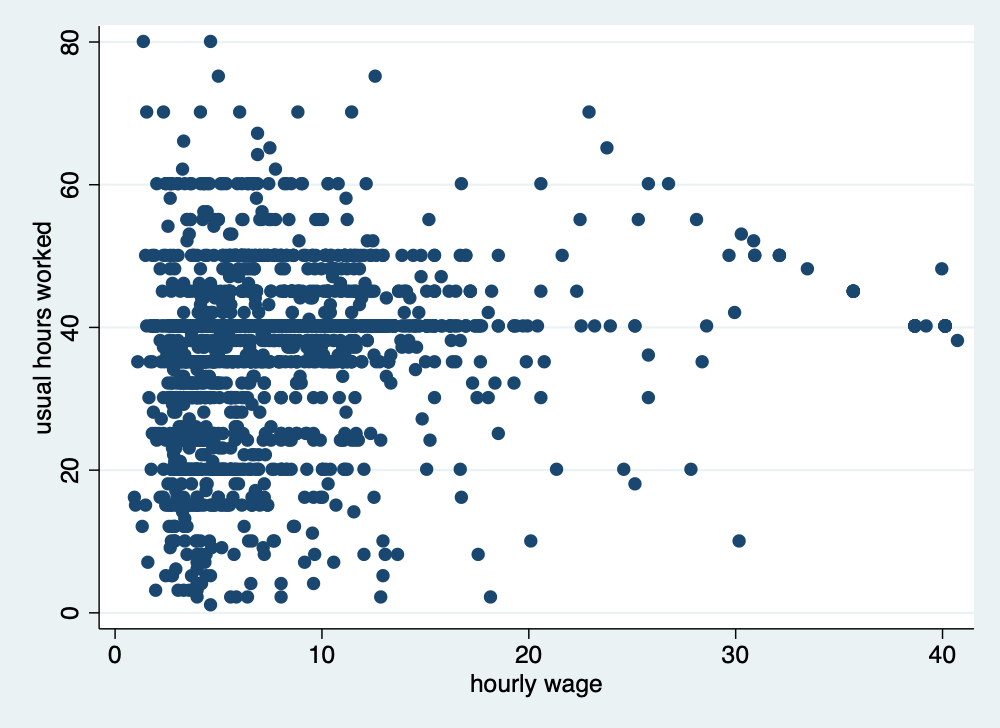
\includegraphics[keepaspectratio,alt={Hours and Wages}]{hour_wage.png}}
\caption{Hours and Wages}
\end{figure}

\section{Fixing and correcting errors in data}\label{fixing-and-correcting-errors-in-data}

Let go ahead and fix some of these errors that we have found. A word of caution is that you may need to talk to the data stewards about the best ways to correct the data. You don't want to attempt to fix the measurement error and introduce additional problems. Institutional knowledge of the data is very helpful before correcting errors.

Let's fix when race was equal to 4 when there are only 3 categories. Let's add a note for future users, which is good practice for replication.

\begin{Shaded}
\begin{Highlighting}[]
\KeywordTok{quietly}\NormalTok{ cd }\StringTok{"/Users/Sam/Desktop/Econ 643/Data/Mitchell"}
\KeywordTok{quietly} \KeywordTok{use}\NormalTok{ wws, }\KeywordTok{clear}
\OtherTok{list}\NormalTok{ idcode race }\KeywordTok{if}\NormalTok{ race==4}
\KeywordTok{replace}\NormalTok{ race=1 }\KeywordTok{if}\NormalTok{ idcode == 543}
\KeywordTok{note}\NormalTok{ race: race changed to 1 (from 4) }\KeywordTok{for}\NormalTok{ idcode 543}
\KeywordTok{tabulate}\NormalTok{ race}
\end{Highlighting}
\end{Shaded}

\begin{verbatim}
      | idcode   race |
      |---------------|
2013. |    543      4 |
      +---------------+

(1 real change made)

       race |      Freq.     Percent        Cum.
------------+-----------------------------------
          1 |      1,637       72.89       72.89
          2 |        583       25.96       98.84
          3 |         26        1.16      100.00
------------+-----------------------------------
      Total |      2,246      100.00
\end{verbatim}

Let's fix college gradudate when there were only 8 years of education.

\begin{Shaded}
\begin{Highlighting}[]
\KeywordTok{quietly}\NormalTok{ cd }\StringTok{"/Users/Sam/Desktop/Econ 643/Data/Mitchell"}
\KeywordTok{quietly} \KeywordTok{use}\NormalTok{ wws, }\KeywordTok{clear}
\OtherTok{list}\NormalTok{ idcode collgrad }\KeywordTok{if}\NormalTok{ yrschool \textless{} 12 \& collgrad == 1}
\KeywordTok{replace}\NormalTok{ collgrad = 0 }\KeywordTok{if}\NormalTok{ idcode == 107}

\KeywordTok{note}\NormalTok{ collgrad: collgrad changed to 0 (from 1) }\KeywordTok{for}\NormalTok{ idcode 107}
\KeywordTok{tab}\NormalTok{ yrschool collgrad}
\end{Highlighting}
\end{Shaded}

\begin{verbatim}
      | idcode   collgrad |
      |-------------------|
2198. |    107          1 |
      +-------------------+

(1 real change made)



  Years of |
    school |   college graduate
 completed |         0          1 |     Total
-----------+----------------------+----------
         8 |        70          0 |        70 
         9 |        55          0 |        55 
        10 |        84          0 |        84 
        11 |       123          0 |       123 
        12 |       943          0 |       943 
        13 |       174          2 |       176 
        14 |       180          7 |       187 
        15 |        81         11 |        92 
        16 |         0        252 |       252 
        17 |         0        106 |       106 
        18 |         0        154 |       154 
-----------+----------------------+----------
     Total |     1,710        532 |     2,242 
\end{verbatim}

Let's fix age which where the digits were switched, and we will make a note of it.

\begin{Shaded}
\begin{Highlighting}[]
\KeywordTok{quietly}\NormalTok{ cd }\StringTok{"/Users/Sam/Desktop/Econ 643/Data/Mitchell"}
\KeywordTok{quietly} \KeywordTok{use}\NormalTok{ wws, }\KeywordTok{clear}
\OtherTok{list}\NormalTok{ idcode age }\KeywordTok{if}\NormalTok{ age \textgreater{} 50}
\KeywordTok{replace}\NormalTok{ age = 38 }\KeywordTok{if}\NormalTok{ idcode == 51}
\KeywordTok{replace}\NormalTok{ age = 45 }\KeywordTok{if}\NormalTok{ idcode == 80}
\KeywordTok{note}\NormalTok{ age: the }\OtherTok{value} \KeywordTok{of}\NormalTok{ 83 was corrected to 38 }\KeywordTok{for}\NormalTok{ idcode 51}
\KeywordTok{note}\NormalTok{ age: the }\OtherTok{value} \KeywordTok{of}\NormalTok{ 54 was corrected to 45 }\KeywordTok{for}\NormalTok{ idcode 80}
\KeywordTok{tab}\NormalTok{ age}
\end{Highlighting}
\end{Shaded}

\begin{verbatim}
      | idcode   age |
      |--------------|
2205. |     80    54 |
2219. |     51    83 |
      +--------------+

(1 real change made)

(1 real change made)

     age in |
    current |
       year |      Freq.     Percent        Cum.
------------+-----------------------------------
         21 |          2        0.09        0.09
         22 |          8        0.36        0.45
         23 |         16        0.71        1.16
         24 |         35        1.56        2.72
         25 |         44        1.96        4.67
         26 |         50        2.23        6.90
         27 |         50        2.23        9.13
         28 |         63        2.80       11.93
         29 |         49        2.18       14.11
         30 |         55        2.45       16.56
         31 |         57        2.54       19.10
         32 |         60        2.67       21.77
         33 |         56        2.49       24.27
         34 |         95        4.23       28.50
         35 |        213        9.48       37.98
         36 |        224        9.97       47.95
         37 |        171        7.61       55.57
         38 |        176        7.84       63.40
         39 |        167        7.44       70.84
         40 |        139        6.19       77.03
         41 |        148        6.59       83.62
         42 |        111        4.94       88.56
         43 |        110        4.90       93.46
         44 |         98        4.36       97.82
         45 |         46        2.05       99.87
         46 |          1        0.04       99.91
         47 |          1        0.04       99.96
         48 |          1        0.04      100.00
------------+-----------------------------------
      Total |      2,246      100.00
\end{verbatim}

Let's look at our notes with the \emph{note} command.

\begin{Shaded}
\begin{Highlighting}[]
\KeywordTok{note}
\end{Highlighting}
\end{Shaded}

\begin{verbatim}
_dta:
  1.  This is a hypothetical dataset and should not be used for analysis purposes

age:
  1.  the value of 83 was corrected to 38 for idcode 51
  2.  the value of 54 was corrected to 45 for idcode 80

race:
  1.  race changed to 1 (from 4) for idcode 543

collgrad:
  1.  collgrad changed to 0 (from 1) for idcode 107
\end{verbatim}

\section{Identifying duplicates}\label{identifying-duplicates}

The duplicates command can be helpful, but it will only find duplicates that are exactly the same \textbf{unless you specify which variables with duplicates list vars}.
We'll cover this a bit later.

We need to be careful with duplicate observations. When working with panel data we will want multiple observations of the same cross-sectional unit, but there should be multiple observations for different time units and not the same time unit.

We can start with our \emph{duplicates} list command to find rows that are completely the same. This command will show all the duplicates. \textbf{Note:} for duplicate records to be found, all data needs to be the same.

\begin{Shaded}
\begin{Highlighting}[]
\KeywordTok{quietly}\NormalTok{ cd }\StringTok{"/Users/Sam/Desktop/Econ 643/Data/Mitchell"}
\KeywordTok{quietly} \KeywordTok{use} \StringTok{"dentists\_dups.dta"}\NormalTok{, }\KeywordTok{clear}
\KeywordTok{duplicates} \OtherTok{list}
\end{Highlighting}
\end{Shaded}

\begin{verbatim}
Duplicates in terms of all variables

  +---------------------------------------------------------+
  | Group   Obs             name   years   fulltime   recom |
  |---------------------------------------------------------|
  |     1     4       Mike Avity     8.5          0       0 |
  |     1     6       Mike Avity     8.5          0       0 |
  |     1     8       Mike Avity     8.5          0       0 |
  |     2     1   Olive Tu'Drill   10.25          1       1 |
  |     2    11   Olive Tu'Drill   10.25          1       1 |
  |---------------------------------------------------------|
  |     3     2     Ruth Canaale      22          1       1 |
  |     3     3     Ruth Canaale      22          1       1 |
  +---------------------------------------------------------+
\end{verbatim}

We'll have a more condensed version with duplicates examples. It will give an
example of the duplicate records for each group of duplicate records.

\begin{Shaded}
\begin{Highlighting}[]
\KeywordTok{duplicates}\NormalTok{ examples }
\end{Highlighting}
\end{Shaded}

\begin{verbatim}
Duplicates in terms of all variables

  +------------------------------------------------------------------+
  | Group   #   e.g. obs             name   years   fulltime   recom |
  |------------------------------------------------------------------|
  |     1   3          4       Mike Avity     8.5          0       0 |
  |     2   2          1   Olive Tu'Drill   10.25          1       1 |
  |     3   2          2     Ruth Canaale      22          1       1 |
  +------------------------------------------------------------------+
\end{verbatim}

We can find the a consice list of duplicate records with duplicates report.

\begin{Shaded}
\begin{Highlighting}[]
\KeywordTok{duplicates} \KeywordTok{report}
\end{Highlighting}
\end{Shaded}

\begin{verbatim}
Duplicates in terms of all variables

--------------------------------------
   Copies | Observations       Surplus
----------+---------------------------
        1 |            4             0
        2 |            4             2
        3 |            3             2
--------------------------------------
\end{verbatim}

The duplicates tag command can return the number of duplicates for each group of duplicates (note the separator option puts a line in the table after \# rows.

\begin{Shaded}
\begin{Highlighting}[]
\KeywordTok{duplicates} \FunctionTok{tag}\NormalTok{, }\KeywordTok{generate}\NormalTok{(dup)}
\OtherTok{list}\NormalTok{, separator(2)}
\end{Highlighting}
\end{Shaded}

\begin{verbatim}
Duplicates in terms of all variables

     +----------------------------------------------------+
     |              name   years   fulltime   recom   dup |
     |----------------------------------------------------|
  1. |    Olive Tu'Drill   10.25          1       1     1 |
  2. |      Ruth Canaale      22          1       1     1 |
     |----------------------------------------------------|
  3. |      Ruth Canaale      22          1       1     1 |
  4. |        Mike Avity     8.5          0       0     2 |
     |----------------------------------------------------|
  5. |        Mary Smith       3          1       1     0 |
  6. |        Mike Avity     8.5          0       0     2 |
     |----------------------------------------------------|
  7. | Y. Don Uflossmore    7.25          0       1     0 |
  8. |        Mike Avity     8.5          0       0     2 |
     |----------------------------------------------------|
  9. |        Mary Smith      27          0       0     0 |
 10. | Isaac O'Yerbreath   32.75          1       1     0 |
     |----------------------------------------------------|
 11. |    Olive Tu'Drill   10.25          1       1     1 |
     +----------------------------------------------------+
\end{verbatim}

Let's sort our data for better legibility, and then we will add lines in our output table whenever there is a new group.

\begin{Shaded}
\begin{Highlighting}[]
\KeywordTok{quietly}\NormalTok{ cd }\StringTok{"/Users/Sam/Desktop/Econ 643/Data/Mitchell"}
\KeywordTok{quietly} \KeywordTok{use} \StringTok{"dentists\_dups.dta"}\NormalTok{, }\KeywordTok{clear}
\KeywordTok{sort} \BaseNTok{name}\NormalTok{ years}
\OtherTok{list}\NormalTok{, sepby(}\BaseNTok{name}\NormalTok{ years)}
\end{Highlighting}
\end{Shaded}

\begin{verbatim}
     |              name   years   fulltime   recom |
     |----------------------------------------------|
  1. | Isaac O'Yerbreath   32.75          1       1 |
     |----------------------------------------------|
  2. |        Mary Smith       3          1       1 |
     |----------------------------------------------|
  3. |        Mary Smith      27          0       0 |
     |----------------------------------------------|
  4. |        Mike Avity     8.5          0       0 |
  5. |        Mike Avity     8.5          0       0 |
  6. |        Mike Avity     8.5          0       0 |
     |----------------------------------------------|
  7. |    Olive Tu'Drill   10.25          1       1 |
  8. |    Olive Tu'Drill   10.25          1       1 |
     |----------------------------------------------|
  9. |      Ruth Canaale      22          1       1 |
 10. |      Ruth Canaale      22          1       1 |
     |----------------------------------------------|
 11. | Y. Don Uflossmore    7.25          0       1 |
     +----------------------------------------------+
\end{verbatim}

\textbf{Notice!} There are two observations for Mary Smith, but one has 3 years of experience and the other one has 27 years, so it does not appear as a duplicate.

If there were too many variables, which could use our data browser.

\begin{Shaded}
\begin{Highlighting}[]
\NormalTok{browse }\KeywordTok{if}\NormalTok{ dup \textgreater{} 0}
\end{Highlighting}
\end{Shaded}

We will want to drop our duplicates, but not the first observation. The duplicates drop command will drop the duplicate records but still keep one observation of the duplicate group.

\begin{Shaded}
\begin{Highlighting}[]
\KeywordTok{duplicates} \KeywordTok{drop}
\end{Highlighting}
\end{Shaded}

Let's use a new dataset that is a bit more practical

\begin{verbatim}
use "wws.dta", replace
\end{verbatim}

Let's check for duplicate idcodes with the \emph{isid command}. If there is a duplicate idcode, the command will return an error.

\begin{Shaded}
\begin{Highlighting}[]
\KeywordTok{quietly}\NormalTok{ cd }\StringTok{"/Users/Sam/Desktop/Econ 643/Data/Mitchell"}
\KeywordTok{use} \StringTok{"wws.dta"}\NormalTok{, }\KeywordTok{replace}
\KeywordTok{isid}\NormalTok{ idcode}
\end{Highlighting}
\end{Shaded}

\begin{verbatim}
(Working Women Survey)
\end{verbatim}

Or just use duplicates list for the variable of interest

\begin{Shaded}
\begin{Highlighting}[]
\KeywordTok{quietly}\NormalTok{ cd }\StringTok{"/Users/Sam/Desktop/Econ 643/Data/Mitchell"}
\KeywordTok{quietly} \KeywordTok{use} \StringTok{"wws.dta"}\NormalTok{, }\KeywordTok{replace}
\KeywordTok{duplicates} \OtherTok{list}\NormalTok{ idcode}
\end{Highlighting}
\end{Shaded}

\begin{verbatim}
Duplicates in terms of idcode

(0 observations are duplicates)
\end{verbatim}

There are no duplicate idcodes, so we should expect that duplicates list will not return any duplicates, since every single values needs to be the same for there to be a dupicate record.

Let's use a dataset that does have duplicates. Let's check for duplicate idcodes.

\begin{Shaded}
\begin{Highlighting}[]
\KeywordTok{quietly}\NormalTok{ cd }\StringTok{"/Users/Sam/Desktop/Econ 643/Data/Mitchell"}
\KeywordTok{use} \StringTok{"wws\_dups.dta"}\NormalTok{, }\KeywordTok{clear}
\KeywordTok{isid}\NormalTok{ idcode}
\end{Highlighting}
\end{Shaded}

\begin{verbatim}
variable idcode does not uniquely identify the observations
r(459);

r(459);
\end{verbatim}

Or

\begin{Shaded}
\begin{Highlighting}[]
\KeywordTok{quietly}\NormalTok{ cd }\StringTok{"/Users/Sam/Desktop/Econ 643/Data/Mitchell"}
\KeywordTok{use} \StringTok{"wws\_dups.dta"}\NormalTok{, }\KeywordTok{clear}
\KeywordTok{duplicates} \OtherTok{list}\NormalTok{ idcode, sepby(idcode)}
\end{Highlighting}
\end{Shaded}

\begin{verbatim}
Duplicates in terms of idcode

  +-----------------------+
  | Group    Obs   idcode |
  |-----------------------|
  |     1   1088     2831 |
  |     1   2248     2831 |
  |-----------------------|
  |     2   1244     3905 |
  |     2   1245     3905 |
  |-----------------------|
  |     3    277     4214 |
  |     3   2247     4214 |
  +-----------------------+
\end{verbatim}

I prefer \emph{duplicates list var1}, since an error will break the do file.

Let's generate our dup variable for identifying the number of duplicates per
group of duplicates.

\begin{Shaded}
\begin{Highlighting}[]
\KeywordTok{duplicates} \FunctionTok{tag}\NormalTok{ idcode, }\KeywordTok{generate}\NormalTok{(iddup)}
\end{Highlighting}
\end{Shaded}

Let's generate a different duplicate variable to find complete duplicate
records. Notice that we do not specify a variable after tag.

\begin{Shaded}
\begin{Highlighting}[]
\KeywordTok{duplicates} \FunctionTok{tag}\NormalTok{, }\KeywordTok{generate}\NormalTok{(alldup)}
\end{Highlighting}
\end{Shaded}

Let's list the data

\begin{Shaded}
\begin{Highlighting}[]
\OtherTok{list}\NormalTok{ idcode age race yrschool occupation wage }\KeywordTok{if}\NormalTok{ iddup==1 \& alldup==0}
\end{Highlighting}
\end{Shaded}

\begin{verbatim}
Duplicates in terms of idcode


Duplicates in terms of all variables

      +------------------------------------------------------+
      | idcode   age   race   yrschool   occupa~n       wage |
      |------------------------------------------------------|
1244. |   3905    36      1         14         11   4.339774 |
1245. |   3905    41      1         10          5   7.004828 |
      +------------------------------------------------------+
\end{verbatim}

It seems that idcode 3905 is a different person with a possible incorrect idcode. Let's fix that.

\begin{Shaded}
\begin{Highlighting}[]
\KeywordTok{replace}\NormalTok{ idcode=5160 }\KeywordTok{if}\NormalTok{ idcode==3905 \& age==41}
\OtherTok{list}\NormalTok{ idcode age race yrschool occupation wage }\KeywordTok{if}\NormalTok{ iddup==1 \& alldup==0}
\end{Highlighting}
\end{Shaded}

\begin{verbatim}
(1 real change made)

      +------------------------------------------------------+
      | idcode   age   race   yrschool   occupa~n       wage |
      |------------------------------------------------------|
1244. |   3905    36      1         14         11   4.339774 |
1245. |   5160    41      1         10          5   7.004828 |
      +------------------------------------------------------+
\end{verbatim}

Let's look observation that are complete duplicates.

\begin{Shaded}
\begin{Highlighting}[]
\KeywordTok{duplicates} \KeywordTok{report}
\OtherTok{list}\NormalTok{ idcode age race yrschool occupation wage }\KeywordTok{if}\NormalTok{ iddup==1 \& alldup==1}
\end{Highlighting}
\end{Shaded}

\begin{verbatim}
Duplicates in terms of all variables

--------------------------------------
   Copies | Observations       Surplus
----------+---------------------------
        1 |         2244             0
        2 |            4             2
--------------------------------------

      +------------------------------------------------------+
      | idcode   age   race   yrschool   occupa~n       wage |
      |------------------------------------------------------|
 277. |   4214    35      1         17         13   11.27214 |
1088. |   2831    37      2          8          8   2.697261 |
2247. |   4214    35      1         17         13   11.27214 |
2248. |   2831    37      2          8          8   2.697261 |
      +------------------------------------------------------+
\end{verbatim}

We need to keep 1 observation of the duplicates. Use the \emph{duplicates drop} command.

\begin{Shaded}
\begin{Highlighting}[]
\KeywordTok{duplicates} \KeywordTok{drop}
\KeywordTok{duplicates} \KeywordTok{report}
\end{Highlighting}
\end{Shaded}

\begin{verbatim}
Duplicates in terms of all variables

(2 observations deleted)


Duplicates in terms of all variables

--------------------------------------
   Copies | Observations       Surplus
----------+---------------------------
        1 |         2246             0
--------------------------------------
\end{verbatim}

\chapter{Exercises}\label{exercises}

Let's work the Census CPS.

Pull the Census CPS.
- You can download the file and import it, or
- You can use Stata to pull the file.

\begin{Shaded}
\begin{Highlighting}[]
\NormalTok{import delimited }\KeywordTok{using} \StringTok{"https://www2.census.gov/programs{-}surveys/cps/datasets/2025/basic/jul25pub.csv"}\NormalTok{, }\KeywordTok{clear}
\end{Highlighting}
\end{Shaded}

Let's save a copy of the csv file in Stata

Let's grab the data dictionary. It can be found here: \url{https://www2.census.gov/programs-surveys/cps/datasets/2026/basic/2026_Basic_CPS_Public_Use_Record_Layout_plus_IO_Code_list.txt}

Import the data and let's check our data.

\begin{enumerate}
\def\labelenumi{\arabic{enumi}.}
\tightlist
\item
  What variable contains our laborforce status?
\item
  What variable contains our weekly earnings?
\item
  Does everyone employed have weekly earnings? Hint: Try \emph{summarize}
\item
  What flag with our weekly earning that provides information about available data?
\item
  Try \emph{tabstat} with the flag and weekly earnings. What do you find?
\item
  Try \emph{tabstat} with statistics(n mean sd p25 p50 p75)
\item
  What are our identifier variable(s)? How many did you find?
\item
  Are there any duplicate records?
\end{enumerate}

Acock, A.C. (2023). A gentle introduction to Stata. 6th ed.~Stata Press.

Anderson, D. R., Sweeney, D. J., Williams, T. A., Camm, J. D., \& Cochran, J. J. (2016). Statistics for business and economics (13th ed.). Cengage Learning.

Mitchell, M. N. (2020). Data management using Stata: A practical handbook. Stata Press.

\bibliography{book.bib,packages.bib}

\end{document}
